\documentclass{article}
\usepackage{mathtools}
\usepackage{tikz}
\usepackage[utf8]{inputenc}
\begin{document}
\section{Dans la peau d'Apollon}
    Les notations: A == Alexandre, R == Robin, M == Miguel, Ae == Alexandrine, F == Floriane
    \begin{itemize}
        \item Les sexes des caractères
            \begin{equation}
            homme(A) \land homme(R) \land homme (M) \land femme(Ae) \land femme(F)
            \end{equation}
        \item Alex est en couple avec Alex et Robin est en couple avec Floriane.
            \begin{equation}
            couple(A, Ae) \land couple(R, F)
            \end{equation}
        \item Il y a une femme et un homme qui aiment leur partenaire respectif mais qui ont aussi des sentiments pour une autre personne.
            \begin{equation}
            \begin{split}
            \exists a, a_1, a_2, b, b_1, b_2 \text{ tel que }(homme(a) \land femme(b) \\
            \land couple(a, a_1) \land aime(a, a_1) \land aime(a, a_2) \\
            \land couple(b, b_1) \land aime(b, b_1) \land aime(b, b_2) \\
            \land a_1 \neq a_2 \land b_1 \neq b_2)
            \end{split}
            \end{equation}
        \item Il y a une femme et un homme qui n’aiment que leur partenaire respectif.
            \begin{equation}
            \begin{split}
            \exists a, a_1, b, b_1,\forall a_2, b_2 \text{ tel que }(homme(a) \land femme(b) \\
            \land couple(a, a_1) \land aime(a, a_1) \land \neg aime(a, a_2) \\
            \land couple(b, b_1) \land aime(b, b_1) \land \neg aime(b, b_2) \\
            \land a_1 \neq a_2 \land b_1 \neq b_2)
            \end{split}
            \end{equation}
        \item \inputencoding{utf8} Après une soirée de folie dans l’épisode 4, Miguel commence à éprouver des sentiments pour une personne qui aime une personne qui aime Alexandrine.
            \begin{equation}
            \exists x, y \text{ tel que } aime(M, x) \land aime(x, y) \land aime(y, Ae)
            \end{equation}
        \item C’est un peu sexiste parce que toutes les femmes n’aiment que des hommes.
            \begin{equation}
            \forall v, v', femme(v, v') \implies \neg aime(v, v')
            \end{equation}
            \begin{equation}
            \text{ ou } \forall v, w, femme(v) \land aime(v, w) \implies homme(w)
            \end{equation}
        \item Robin aime une personne dans un triangle amoureux.
            \begin{equation}
            \exists d, e \text{ tel que } aime(Robin, d) \land aime(d, e) \land aime(e, Robin)
            \end{equation}
        \item Personne ne s’aime soi-même.
            \begin{equation}
            \forall x, \neg aime(x, x)
            \end{equation}
    \end{itemize}
    Une graphe de relation qui satisfait (1) à (9):
    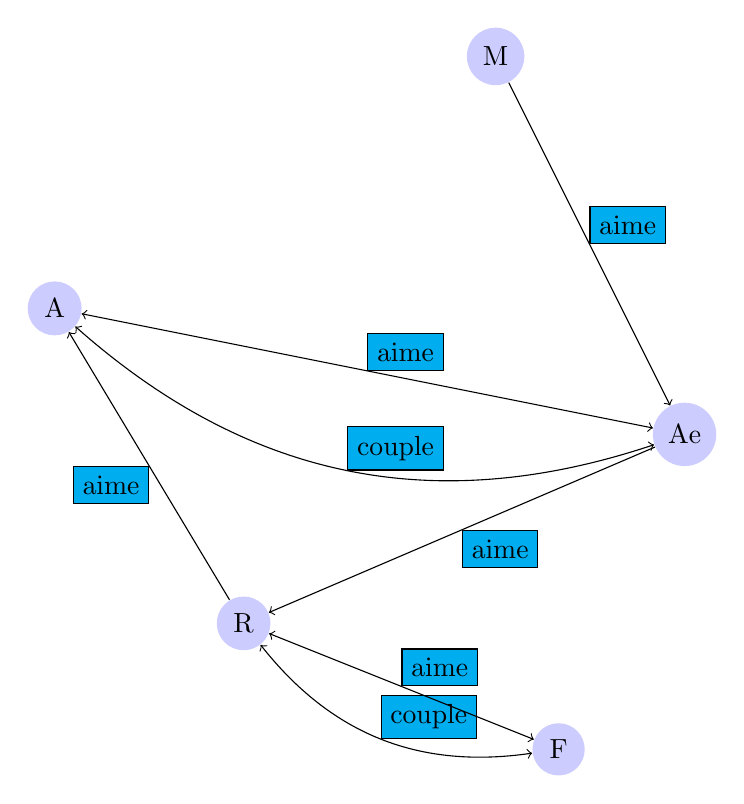
\begin{tikzpicture}
        [scale=.8,auto=left,every node/.style={circle,fill=blue!20}]
        \node (Alexandre) at (1,10) {A};
        \node (Robin) at (4,5)  {R};
        \node (Miguel) at (8,14)  {M};
        \node (Alexandrine) at (11,8) {Ae};
        \node (Floriane) at (9,3)  {F};
        \tikzset{LabelStyle/.style =   {draw,
                                  shape          = rectangle,
                                  fill           = cyan,
                                  text           = black}}
        \foreach \from/\to in {Alexandre/Alexandrine,Robin/Floriane}
            \draw[<->, bend right] (\from) to node[LabelStyle]{couple} (\to);
        \foreach \from/\to in {Alexandre/Alexandrine,Robin/Floriane}
            \draw[<->] (\from) to node[LabelStyle]{aime} (\to);
        \foreach \from/\to in {Miguel/Alexandrine, Robin/Alexandre, Alexandrine/Robin}
            \draw[->] (\from) to node[LabelStyle]{aime} (\to);
    \end{tikzpicture}
\section{Saison 2}
    L'assertion représenté en utilisant les séquents (note: Alex peut représenter Alexandre OU Alexandrine):
    \begin{displaymath}
    \begin{split}
    (1), ..., (9), \forall m, homme(m), \text{frère}(Alex, m) \vdash ([aime(Alex, m) \land aime(M, F)], \\
    [\neg aime(Alex, m) \land \neg aime(M, F)])
    \end{split}
    \end{displaymath}
    Je vais utiliser le cas où Alex = Alexandre = A, et où j'ai choisit pour m = Robin
    \begin{displaymath}
    (1), ..., (9), \text{frère}(A, R) \vdash [aime(A, R) \land aime(M, F)], [\neg aime(A, R) \land \neg aime(M, F)]
    \end{displaymath}
    Vu qu'on a des AND après le turnstile, on a plusieurs branches possibles, choisissant aime(M, F) 
    \begin{displaymath}
    (1), ..., (9), \text{frère}(A, R) \vdash aime(M, F), [\neg aime(A, R) \land \neg aime(M, F)]
    \end{displaymath}
    Comme on ne peut pas avoir aime(M, F) et not aime(M, F) comme hypothèse en même temps, on peut représenter la deuxième possibilité par un delta maj.:
    \begin{displaymath}
    (1), ..., (9), \text{frère}(A, R) \vdash aime(M, F), \Delta
    \end{displaymath}
    Un des possibles reduction de l'hypothèse (note: pour réduire la longeur, la relation couple représente aussi une amour bidirectionelle, car (2) et (3) ,ensemble , demadent toujours que tous les personnes dans les 2 paires aime son partenaire) pour avoir inceste (pour satisfaire l'hypothèse initiale):
    \begin{displaymath}
    \begin{split}
    couple(A, Ae), couple(R, F), aime(F, A), \text{frère}(A, R), aime(A, R), (aime(M, F) \\
    \lor aime(M, Ae)) \vdash aime(M, F), \Delta
    \end{split}
    \end{displaymath}
    Si on choisit aime(M, Ae), on trouvera que l'hypothèse est fausse:
    \begin{displaymath}
    couple(A, Ae), couple(R, F), aime(F, A), \text{frère}(A, R), aime(A, R), aime(M, Ae) \vdash aime(M, F), \Delta
    \end{displaymath}
    C'est fausse car l'hypothèse ne demande pas que Miguel aime Floriane
\end{document}

